\textbf{Taller con el Brazo Robótico SCORBOT-ER 4u}

Tomando como referencia el Brazo SCORBOT-ER 4u disponible en el laboratorio. Investigue sobre las características de este brazo e identifique los grados de libertad e intente identificar qué tipo de articulaciones encontramos en el Brazo SCORBOT-ER 4u. Utilizar recursos de apoyo como videos en la Web. 

\begin{figure}[H]
    \centering
    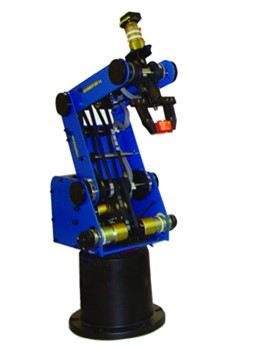
\includegraphics[scale = 0.5]{Imagenes/robot_p1.jpg}
    \caption{Figura1: Brazo SCORBOT-ER 4u }{Fuente: Profesor}
\end{figure} 